\section{Environment Models}
Within this work, we will encounter several different regions of the space environment -- This section provides a collected overview of each region and the models used.
\subsection{Magnetic Field}
\paragraph{Magnetic Dipole}
\paragraph{IGRF}
\paragraph{Tsyganenko Corrections}
\subsection{Ionosphere}
\paragraph{IRI}

\subsection{Plasmasphere}
The plasmasphere is a region of the space environment surrounding the Earth, and a primary unknown within our modeling. The plasmasphere extends from an altitude of ~1000km up to several Earth radii; typically it is divided into two separate regions: a dense, relatively cold \emph{inner plasmasphere}, and a sparse, relatively hot \emph{outer plasmasphere} or \emph{trough}. The transition boundary between the two regions is a sharp dropoff in plasma density called the \emph{plasmapause}.

Much like the ionosphere, the plasmasphere is a highly variable region, depending on solar conditions ($K_p$), location (latitude, longitude, field line), and time of day (MLT). The large spatial scales, high variability, and sparse availability of in-situ measurements require us to turn to empirical models of each region. We consider three primary models of electron density, and two of electron temperature.

\subsubsection{Overview of Plasmasphere Density Models}

\paragraph{Ngo Model}

The Ngo model is a legacy model used extensively in research at Stanford from the early 1980s through the mid-2000s, notably by \cite{Lauben1998} and \cite{Bortnik2005}, and has heritage dating back to the early days of radioscience at Stanford \citep{Kimura1966} The model uses a Diffusive Equilibrium (DE) model for the inner and outer plasmasphere, onto which the \cite{Carpenter1992} inner plasmasphere model is overlaid. This model was integrated into the legacy Stanford VLF raytracing code, and provided several adjustable parameters, including plasmapause location, constituent ratios, and the ability to include ducts.

\paragraph{Global Core Plasmasphere Model}

The Global Core Plasmasphere Model (GCPM), initially developed in 2000 by \cite{Gallagher1999} with significant updates through the following decade, smoothly transitions between several regional models to provide a continuous model of the plasmasphere. Within this work we use version 2.4, which was released in 2009 and made available by the Space Plasma Physics group at the NASA Marshall Space Flight Center (https://plasmasphere.nasa.gov). GCPM incorporates the \cite{Carpenter1992} inner plasmasphere model and the \cite{Gallagher1995} outer plasmasphere model, with an empirical fit of the plasmapause location between. The polar cap model is derived from \cite{Persoon1983} and \cite{Chandler1991}. All models are connected smoothly to the IRI model of the ionosphere at lower altitudes. The combined GCPM model is parameterized by $K_p$ and MLT.

\paragraph{Simplified GCPM}

GCPM aims to provide a dynamic, complete picture of the plasmasphere as a function of time and $K_p$; however for our purposes GCPM provides too much variation. Additionally, the combination and smoothing between many models is computationally slow. In order to provide quicker computation and to reduce the number of parameters to adjust, we have implemented a simplified version of GCPM.

This model uses the equatorial-plane GCPM model, including the plasmapause location. However we omit any variation along latitude, and assume densities are constant along each field line. As our region of interest lies primarily within low and mid latitudes, we omit the polar cap model altogether and simply merge the ionosphere into the equatorial trough model. Finally to simplify computation, we model the ionosphere using an empirical fit to IRI -- one for noon, and one for midnight, with a smooth transition along longitude.

Figure \ref{fig:plasma_model_comparison} shows a side-by-side comparison of the three models.
\begin{figure}[h]
\begin{center}
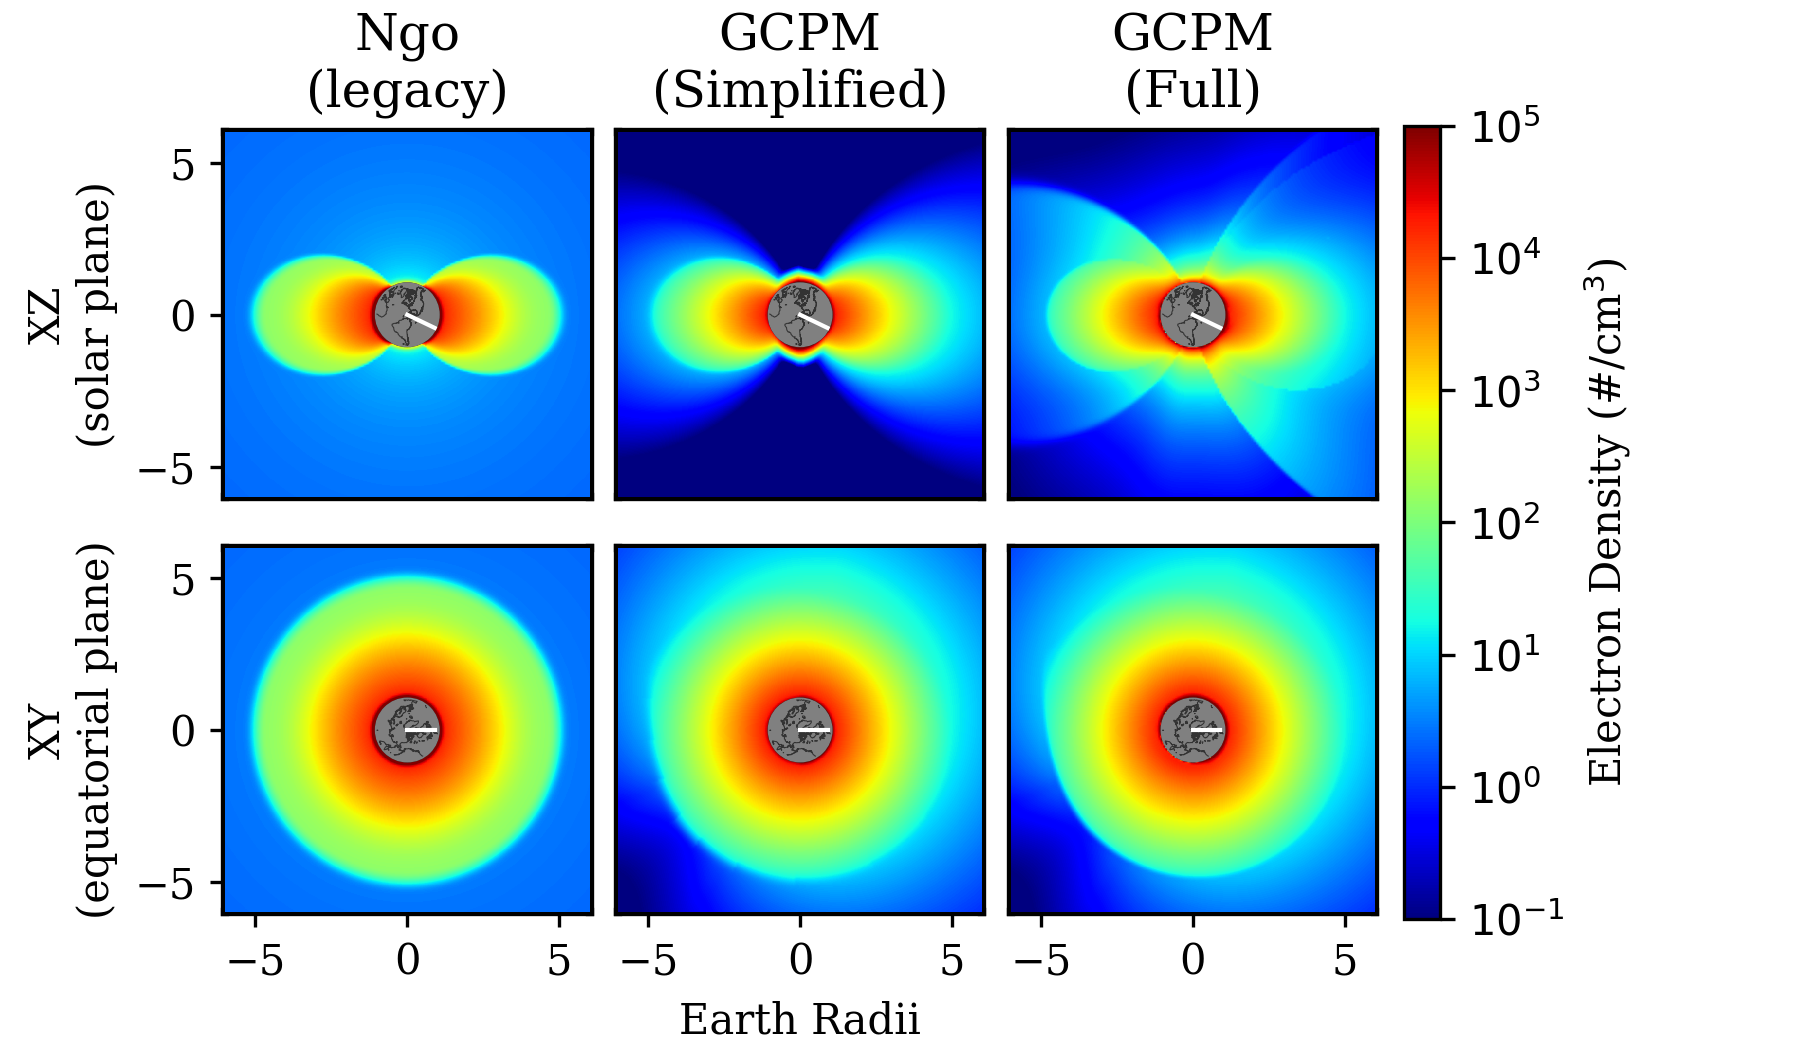
\includegraphics{figures/plasma_model_comparison_serif.png}
\caption{A comparison of three plasmasphere models: Ngo, simplified GCPM, and full GCPM, for a relatively quiet plasmasphere ($K_p=2$). The top row shows electron density in-plane with the direction of solar influx; the bottom row shows a top down (equatorial cross-section) view. The white line indicates the solar axis. Only electron density is shown, as additional plasma constituents are derived from electron density.}
\label{fig:plasma_model_comparison}
\end{center}
\end{figure}